\documentclass[10pt,a4paper]{article}
\usepackage[margin=0.8in]{geometry}
\usepackage{graphicx,booktabs,amsmath,enumitem,microtype,float}
\usepackage[colorlinks=true,urlcolor=blue,linkcolor=black]{hyperref}
\setlist{nosep,leftmargin=1.4em}
\setlength{\parindent}{0pt}\setlength{\parskip}{3pt}
\renewcommand{\arraystretch}{1.05}

\title{\vspace{-1.2em}\textbf{Forecasting short-term 2.4~GHz channel occupancy from sparse RF monitoring:\\
an exploratory study on public AERPAW measurements}\vspace{-0.4em}}
\author{Art Wieczorkowski \quad\textit{Research note, October 2026}}
\date{}

\begin{document}
\maketitle
\vspace{-1.6em}

\textbf{Summary.} Using two public sweep sessions (urban node CC1 and rural node LW1, 87--6019~MHz,
February 2022), I forecast the \emph{fraction of observed sweeps detected busy in the 2.4~GHz channel-6 band} (activity
consistent with Wi-Fi, not decoded) over the next 5, 15 and 60 minutes, and measure how forecast quality
degrades when evidence is dropped, interrupted or delayed. Three results matter most.
(1)~\textbf{Evidence ages quickly}: for a short-memory estimator, skill halves when the newest sweep is
45--80~min old. (2)~\textbf{``Busy'' depends on calibration}: a $\sim$1~dB noise-floor difference changes the
busy prevalence by 2--25$\times$. (3)~Skill comes mostly from tracking the slowly varying activity level; learned
models never clearly beat tuned moving averages, but they were trained on only 2--5 days and each evaluation
set holds only about 33--72 effective independent windows, so this is weak evidence about learning itself.
Protocols were written before the corresponding evaluations according to the project record;
independent registration timestamps are not provided. LW1 channel selection overlaps its first scored fold; two of four, one of four and one of four planned predictions failed, and are reported as such.

\section*{1\quad Question and scope}
\textit{How accurately can short-term spectrum occupancy be predicted from real monitoring records, and
how do observation age and missing measurements affect reliability?} The work stops at occupancy
prediction: it involves no graph or multi-agent learning and no transmission. ``Busy'' means \emph{detected power above a
threshold at one sensor}; it is not transmitter activity, interference elsewhere, or permission to
transmit, and a predicted-idle channel is not evidence that using it would be harmless.

\section*{2\quad Data and provenance}
AERPAW fixed-node sub-6~GHz sweeps (Dryad \href{https://doi.org/10.5061/dryad.hmgqnk9zn}{10.5061/dryad.hmgqnk9zn},
CC0): one SigMF pair per sweep, 98{,}868 bins, power in dBm per 60~kHz bin (calibration undocumented, so only
relative levels are used). Archives were checked against the published SHA-256. CC1: 7.0~days gap-free,
sweeps every 19~s; LW1: 4.75~days gap-free, every 30~s. The NIST COVID-19 occupancy release
(doi:10.18434/mds2-2553) was my first choice because its sensing is natively sparse (77\,\% dead time),
but its file server returned errors throughout the project, so it was not used. Consequently
\textbf{sparsity here is simulated}, by degrading the predictor's inputs; labels always come from the
intact stream. Synthetic data are used only for tests and a separate workflow demo. Controls (\texttt{docs/sanity\_checks.md}): the busy rule fires on $\le0.06\,\%$ of sweeps in idle 5~GHz bands, receiver drift is $\approx0.1$~dB, and the busy state is a bump on the 2430--2445~MHz blocks ($+2.7$ to $+3.5$~dB) that vanishes outside the channel, as a $\sim$20~MHz emitter would produce; nothing was decoded, so ``Wi-Fi'' is an inference.

\section*{3\quad Target and protocol}
Busy sweep: 20~MHz band-mean power (linear average) $>$ noise floor $+\,3$~dB, the floor being the 5th
percentile of the \emph{training period} per channel. Target: fraction of observed sweeps labeled busy in the window
$[o,o{+}W)$, $W\in\{5,15,60\}$~min, forecast at origin $o$ from sweeps that ended before $o$ (minus any
delay). Features are causal and age-aware (decayed and windowed busy fractions, linear-mean power,
time since the last sweep, cross-channel state; missing evidence is NaN plus an age, never zero power
or ``idle''). Baselines: train mean, hour-of-day prior, busy fraction of the last 5~min / 30~min / 2~h,
decayed history; learned: ridge, gradient boosting, and ``last 2~h + learned correction''.
Chronological splits use an embargo of look-back plus $W$. CC1: development region = first 75\,\% of
the week (three rolling one-day folds); the last 1.77~days were evaluated \emph{once} after freezing the
design and writing predictions (\texttt{docs/test\_protocol.md}); a lock file and a code fingerprint
guard the script. LW1 used the design fixed on CC1; its channel-selection period (first 60\,\%, to day 2.85) overlaps the first scored fold [2,3) days, limiting independent confirmation.
Uncertainty: block bootstrap over 2~h blocks; robustness is averaged over five random masks. A transfer analysis fits models on one node (alone, or on both) and forecasts the other, with every node's training data cut at the same time so that simultaneous recordings cannot leak (\texttt{docs/transfer\_protocol.md}, predictions written beforehand).

\section*{4\quad Results}
\begin{center}\small
\begin{tabular}{@{}lccc@{}}\toprule
RMSE of the 15-min busy-fraction forecast & CC1 dev (3 folds) & CC1 test & LW1 (3 folds)\\\midrule
Train mean (climatology) & 0.121 & 0.170 & 0.101\\
Last 2\,h average & \textbf{0.066} & 0.095 & 0.081\\
Last 30\,min average & 0.066 & 0.080 & \textbf{0.073}\\
Decayed history (15\,min) & 0.067 & \textbf{0.078} & 0.075\\
Ridge & 0.092 & 0.083 & 0.074\\
Gradient boosting & 0.085 & 0.126 & 0.077\\\bottomrule
\end{tabular}\\[2pt]
{\footnotesize Table 1. Lower is better. Windows: 307 / 169 / 261. Within-fold $R^2$ of the best method:
0.51 / 0.79 / 0.22.}
\end{center}

\begin{center}\small
\begin{tabular}{@{}lp{5.4cm}p{7.4cm}@{}}\toprule
 & Registered claim & Outcome\\\midrule
CC1 H1 & No learned model beats the 2\,h average by $>0.10$ & \textbf{Rejected}: ridge $+0.24$
[$+0.01,+0.33$], but boosting $-0.76$; the non-learned decayed history is best ($+0.33$)\\
CC1 H2 & Hour-of-day prior has $R^2<0$ & \textbf{Rejected} ($+0.04$)\\
CC1 H3 & Robustness ordering of methods & Supported (all parts)\\
CC1 H4 & Test level higher than last dev day & Supported (0.191 vs 0.096)\\
LW1 N1 & No learned model beats best simple history by $>0.10$ & Supported (ridge $-0.01$)\\
LW1 N2 & Boosting worse than the 2\,h average & \textbf{Rejected} ($+0.10$ [$-0.34,+0.27$])\\
LW1 N3 & Clean-trained ridge least robust & Supported (4 of 4 scenarios)\\
LW1 N4 & LW1 quieter than CC1 & Supported (0.073 vs 0.17--0.20)\\
Transfer T1 & History averages unaffected by training node & Supported (penalty 1.00)\\
Transfer T2 & Ridge, boosting lose when trained on the other node & Supported (MSE $3.7\times$, $2.6\times$)\\
Transfer T3 & Level-anchored (residual) models transfer better & Supported ($1.9\times$ vs $3.7\times$; $1.3\times$ vs $2.6\times$)\\
Transfer T4 & Adding the other node gives no gain & \textbf{Rejected} (boosting $0.94$ [$0.85,1.03$])\\\bottomrule
\end{tabular}\\[2pt]
{\footnotesize Table 2. Skill is relative to the reference named in the claim; intervals are 95\,\% block-bootstrap.}
\end{center}

\textbf{Findings.}
(i)~\emph{Evidence ages within about an hour.} The 15-min-window skill (vs train mean) of the decayed-history
estimator halves when the newest sweep is 78, 57 and 44~min old (CC1 dev, CC1 test, LW1); a 2\,h average halves at
$>120$, 72 and 32~min, and boosting keeps most of its skill at 2\,h (it uses time of day).
(ii)~\emph{Calibration.} Labelling a node with the \emph{other} node's absolute dBm thresholds (floors differ by
$\sim$1~dB) changes its busy prevalence by 2--25$\times$.
(iii)~\emph{Level tracking.} Single sweeps are nearly unpredictable (lag-1 autocorrelation $\approx0.15$); the window
busy share is predictable mostly from the recent level (within-region $R^2$ of the best method 0.51 / 0.79 / 0.22).
(iv)~\emph{Models vs averages.} Learned models never clearly beat the best simple history; boosting was clearly worse
on CC1 but not on LW1 (cause unknown); the best memory length changed (2\,h on CC1 dev, 30\,min/decayed on CC1 test
and LW1). The intervals are probably too narrow (window autocorrelation 0.57--0.67 at 15\,min and still 0.47 on CC1, 0.23 on LW1, at 2\,h).
(v)~\emph{Robustness} (CC1 test): with 90\,\% of sweeps dropped the 2\,h average keeps skill $0.59$, ridge $0.37$; at
99\,\% they are $-1.23$ and $-10.5$ while boosting stays at $+0.14$. Simple averages degrade gracefully; a
clean-trained linear model is unstable.
(vi)~\emph{Transfer} (CC1$\to$LW1, 15~min; \texttt{docs/transfer\_results.md}): history averages $1.00\times$ MSE, ridge
$3.7\times$, boosting $2.6\times$, ``last 2\,h + correction'' $1.3$--$1.9\times$; pooling both nodes is about neutral;
linear models transfer badly in both directions.

\section*{5\quad Limits}
Two nodes (CC1: 7.0 days; LW1: 4.75), one band; only 2--5 training days and roughly 33--72 effective
independent evaluation windows. Rankings are unresolved and intervals may be too narrow. Sparsity
is simulated; power is uncalibrated and sweep hop dwell is unknown. Sweep fractions are not measured
duty cycles. Window targets, rolling folds and the 2\,h reference were chosen after viewing development
scores. Equal-false-busy comparisons use evaluation-label oracle thresholds, not deployment thresholds.

\clearpage
\begin{figure}[H]\centering
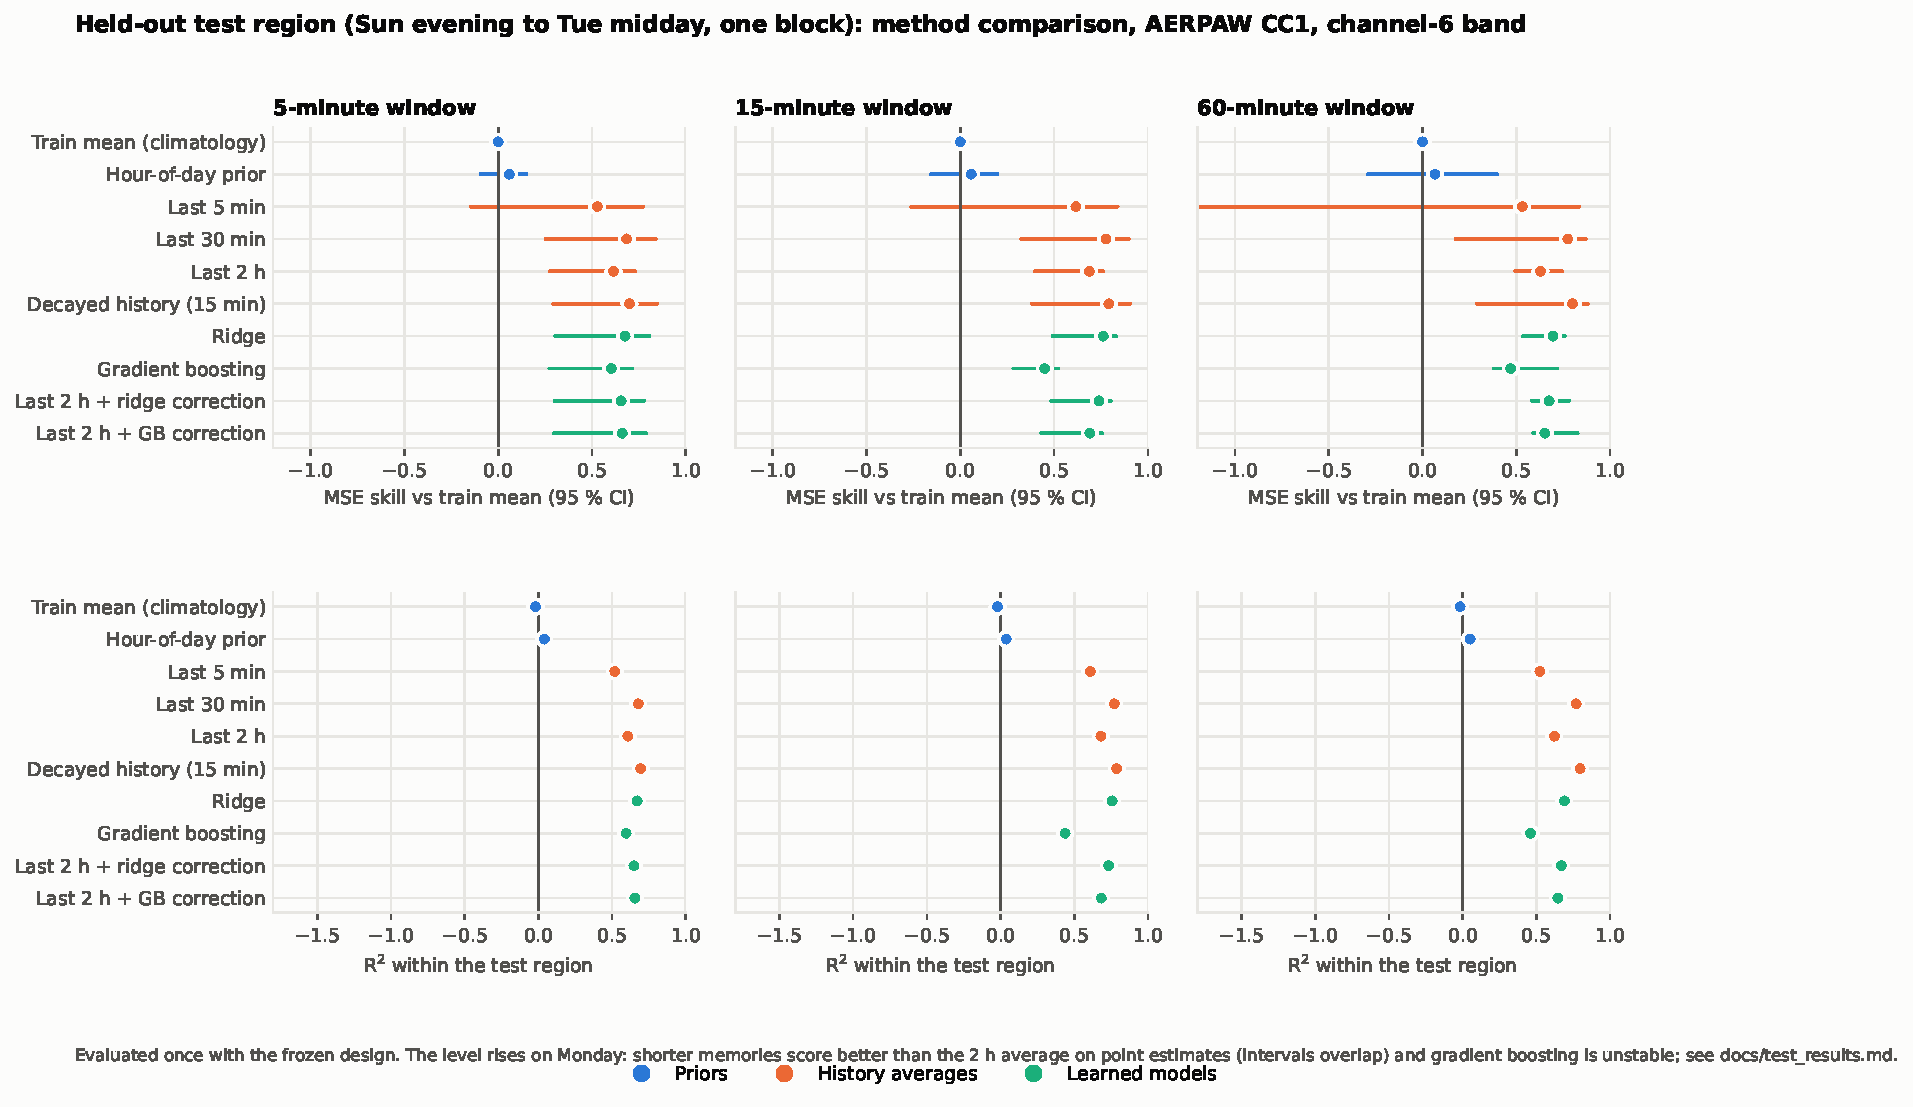
\includegraphics[width=0.74\linewidth]{../../results/figures_test/fig2_method_comparison.pdf}
\caption{\footnotesize Held-out CC1 test region: method comparison for 5/15/60-min windows
(top: MSE skill vs train mean with 95\,\% CI; bottom: $R^2$ within the test region).}
\end{figure}
\begin{figure}[H]\centering
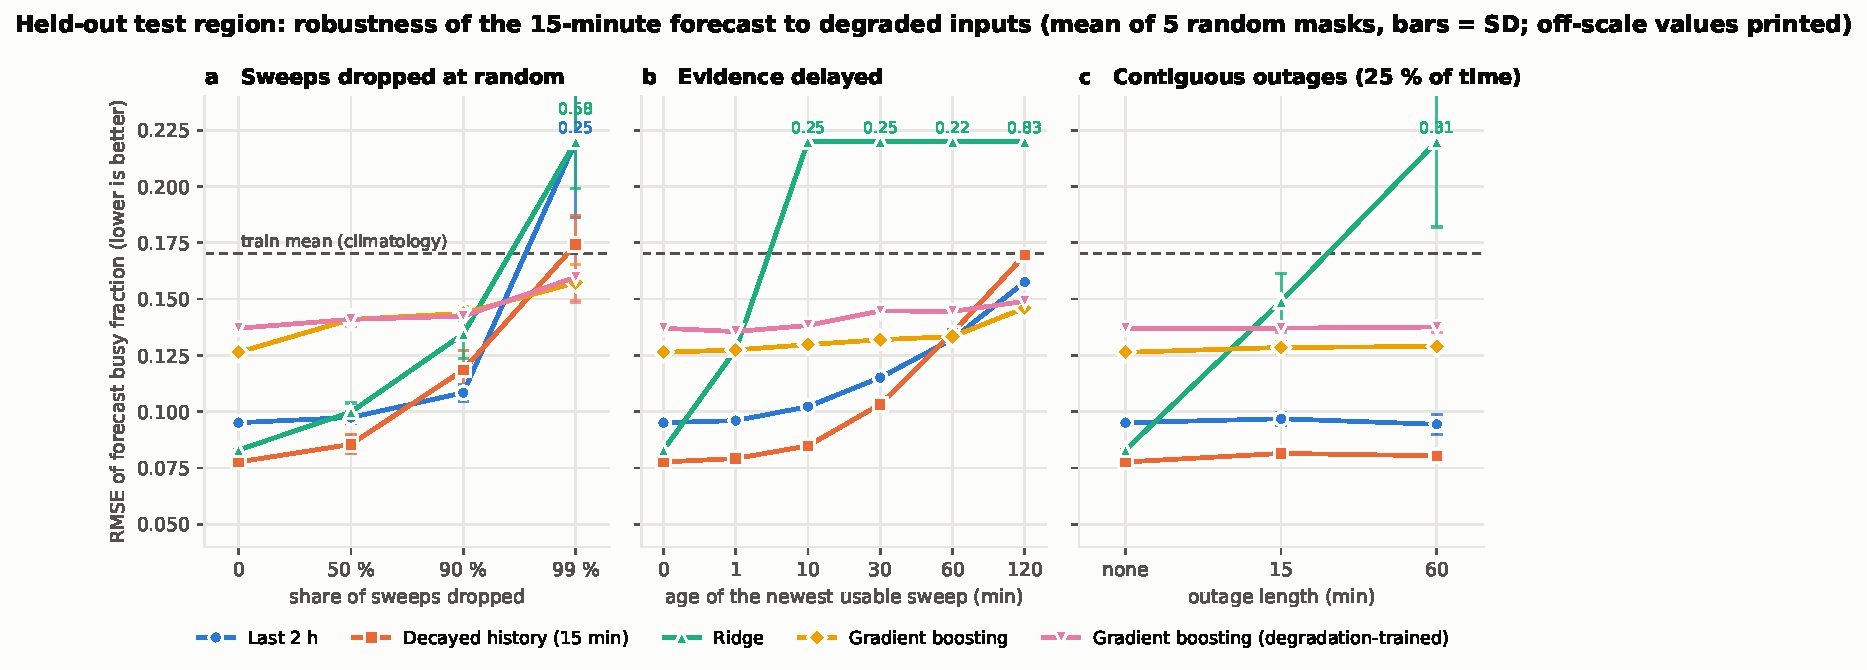
\includegraphics[width=0.74\linewidth]{../../results/figures_test/fig3_robustness.pdf}
\caption{\footnotesize Held-out CC1 test region: RMSE of the 15-min forecast under random sweep loss,
delayed evidence and contiguous outages (mean of 5 masks, bars = SD).}
\end{figure}

\section*{6\quad Open questions}
\begin{enumerate}
\item \textbf{Occupancy semantics.} Is a noise-floor-relative detection threshold the right definition, or should
occupancy be defined against calibrated, regulatory-style thresholds? A 1~dB floor difference reshapes the busy
label, so cross-site comparability needs calibrated data.
\item \textbf{Forecast interface.} Should a downstream controller consume a busy-fraction forecast with
uncertainty, or the raw age-aware evidence (value, age, availability mask) so that staleness stays explicit?
\item \textbf{Non-stationarity.} Since the best memory length is unstable, would adaptive or change-point methods,
or uncertainty-aware abstention under distribution shift, do better?
\item \textbf{Native sparsity and multiple sites.} Do datasets with natively irregular or budget-limited sampling
and several co-located sensors show the same evidence-ageing behaviour as the simulated gaps used here?
\end{enumerate}

\textbf{Reproducibility.} Commands: \texttt{docs/reproduction.md}. Code, original protocols,
historical locks, results and plots are in the repository. New hashes use repository-relative paths;
original locks are preserved and do not independently establish registration chronology. Data are
not redistributed (CC0 source above).
\end{document}
